\documentclass[a4paper]{article}
\usepackage[affil-it]{authblk}
\usepackage[backend=bibtex,style=numeric]{biblatex}
\usepackage{amsmath,amsthm,amssymb}
\usepackage{array}
\usepackage{geometry}
\usepackage{comment}
\usepackage{graphicx}
\geometry{margin=1.5cm, vmargin={0pt,1cm}}
\setlength{\topmargin}{-1cm}
\setlength{\paperheight}{29.7cm}
\setlength{\textheight}{25.3cm}

\addbibresource{citation.bib}


\begin{document}
% =================================================
\title{Report two}

\author{HuiyiLi 12435055
  \thanks{Electronic address: \texttt{lililihuiy@163.com}}}
\affil{(Computational mathematics , Second class of 24th PHD), Zhejiang University }


\date{Due time: \today}

\maketitle
 \begin{abstract}
  Newton interpolation, Hermite interpolation, and cubic Bezier curves are introduced in sections A, B, and F, respectively. The solutions to the other problems are explained in each section, and the final image displays all the results.
\end{abstract} 


\section{A}
Function.hpp contains an abstract function class, which includes two member functions: one is an overloaded  operator(), and the other is derivative() for computing the derivative.

interpolation.cpp implements Newton's interpolation formula. It takes as input the known interpolation nodes x, the corresponding values y, the number of nodes n,
and the point to$\_$inter where you want to calculate the value. The output is the interpolated value out$\_$put.

\section{B}
In Problem B, the class F1 is defined to inherit from the abstract class Function. Polynomial interpolation is performed in four different scenarios, 
and the results are compared with the original function through plotting. As the number of interpolation nodes increases, Runge's phenomenon occurs.
\begin{figure}[htbp]
  \centering
  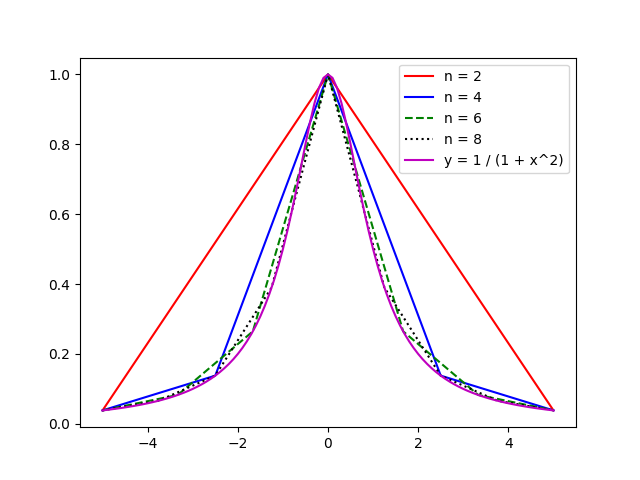
\includegraphics[width=0.6\textwidth]{B.png}
  \caption{B}
  \label{B}
\end{figure}

\section{C}
In Problem C, the class F2 is defined to inherit from the abstract class Function. Polynomial interpolation is performed in four different scenarios, 
and the results are compared with the original function through plotting. Using Chebyshev interpolation can avoid Runge's phenomenon.
\begin{figure}[htbp]
  \centering
  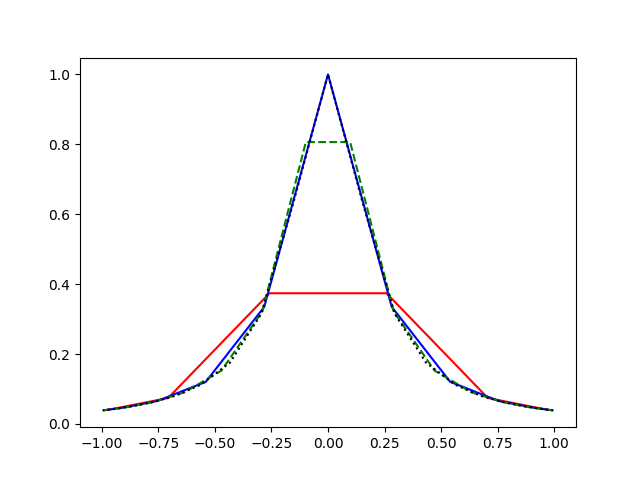
\includegraphics[width=0.6\textwidth]{C.png}
  \caption{C}
  \label{C}
\end{figure}

\section{D}
The hermite.hpp file contains an interpolation node class and two functions. The hermite{\_}Node class consists of interpolation nodes x, node function values f,
 and corresponding derivative values df. The hermite{\_}diag() function takes an instance of the interpolation node class as input and outputs the coefficient
vector for the Hermite interpolation. The hermite{\_}output() function, given the coefficient vector, an instance of the interpolation node class, and an evaluation point, outputs the value of the interpolation polynomial at that point.

\subsection*{a}
Using Hermite interpolation, the predicted position of the car at $t=10s$ is $742.503 feet$, and the velocity is $48.3817 feet/s$.
\subsection*{b}
From the following picture, we get that the first overspeed is at the time of 6s!
\begin{figure}[htbp]
  \centering
  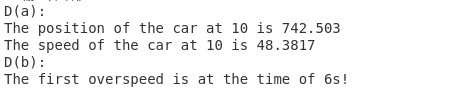
\includegraphics[width=0.6\textwidth]{D.png}
  \caption{D}
  \label{D}
\end{figure}
\section{E}
\subsection*{a}
The following picture shows the shows the average weight curve of these two samples.
\begin{figure}[htbp]
  \centering
  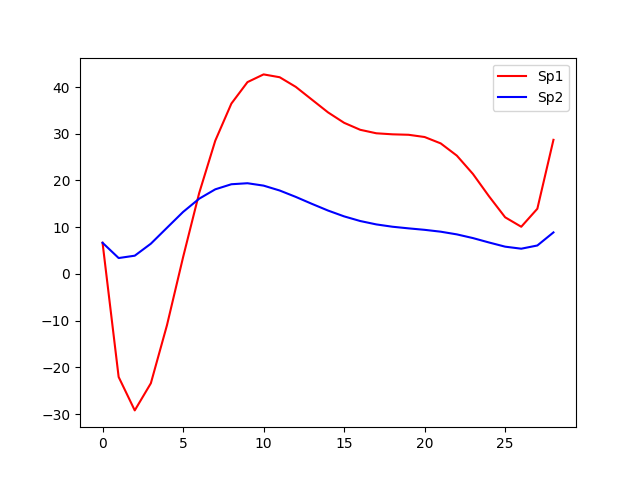
\includegraphics[width=0.6\textwidth]{E(a).png}
  \caption{E}
  \label{E}
\end{figure}
\subsection*{b}
In ProblemE.cpp, after predicting the weight of the two samples over the next 15 days and comparing it to $0$, both of the two samples will not die.

\section{F}
In Bezier.hpp, the function Bezier() takes four nodes $p0,p1,p2,p3$,and the number of points needed to draw the Bezier curve as input, and outputs a vector of points on the Bezier curve.

In ProblemF.cpp, heart{\_}Points() returns a vector of points on a heart-shaped curve based on the number of input points. tan{\_}Vectors() outputs the tangent vector at a given point on the heart-shaped curve.
 Fit() takes points, tangent vectors, and an interval as input to output the fitted Bezier curve values, where the interval controls the number of points uesd for generating the Bezier curve.

 The results for the three cases are shown below:
 \begin{figure}[htbp]
  \centering
  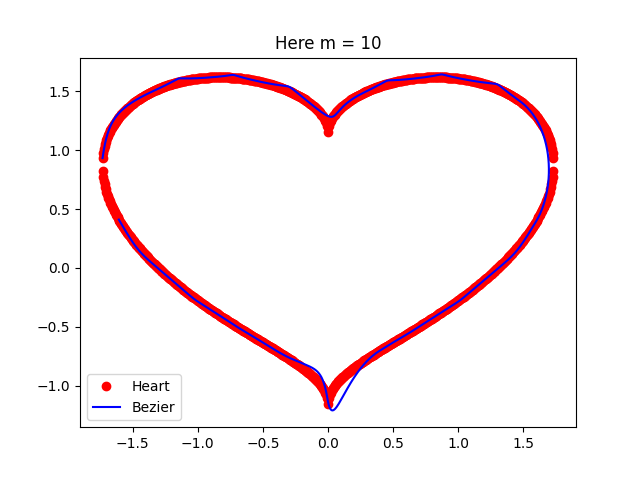
\includegraphics[width=0.6\textwidth]{F1.png}
  \caption{m = 10}
\end{figure}
\begin{figure}[htbp]
  \centering
  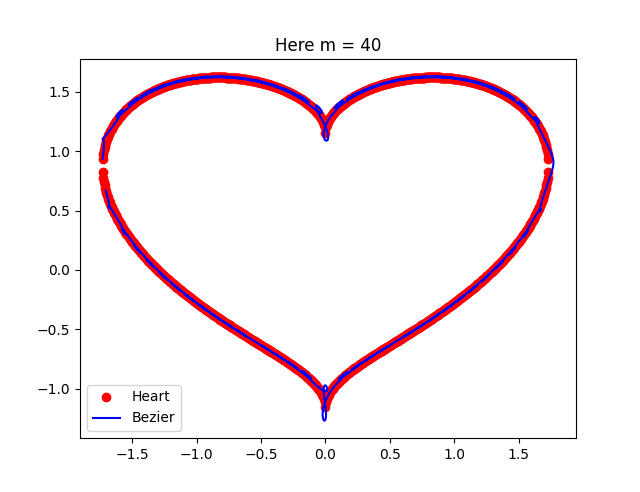
\includegraphics[width=0.6\textwidth]{F2.png}
  \caption{m = 40}
\end{figure}
\begin{figure}[htbp]
  \centering
  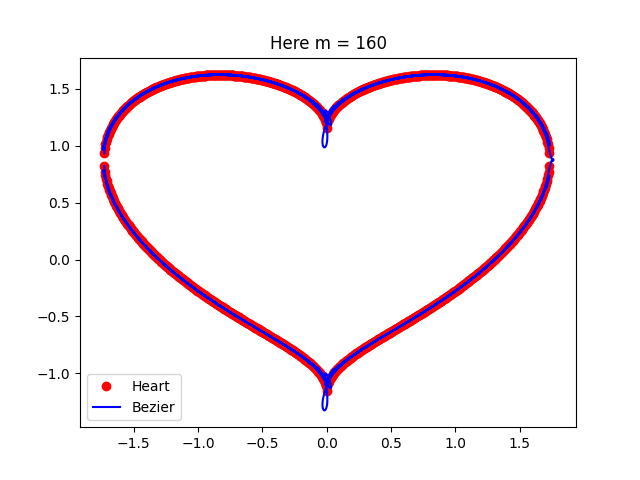
\includegraphics[width=0.6\textwidth]{F3.png}
  \caption{m =160}
\end{figure}

\section*{Result}
Here is all results.
\begin{figure}[htbp]
  \centering
  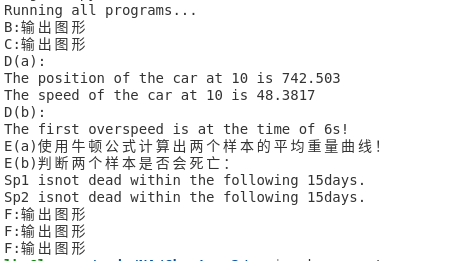
\includegraphics[width=0.6\textwidth]{result.png}
  \caption{All}
\end{figure}


\end{document}


